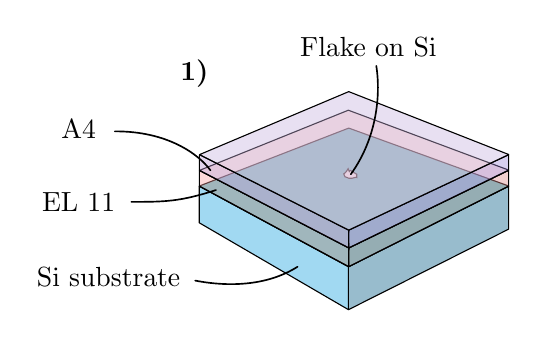
\begin{tikzpicture}

  \draw[line join=bevel, fill=cyan!89!violet!40] (-0.248,1.4) -- (-0.248,0.934) -- (1.648,-0.17) -- (1.648,0.375) -- cycle;
  \draw[line join=bevel, fill=cyan!87!purple!34!lightgray] (1.645,0.376) -- (3.68,1.4) -- (3.68,0.853) -- (1.645,-0.17) -- cycle;
  \draw[fill=teal!90!blue!68!cyan, line join=bevel, draw opacity=1, fill opacity=0.6] (-0.25,1.4) -- (1.65,2.137) -- (3.685,1.4) -- (1.65,0.377) -- cycle;  \draw[fill=white, rounded corners=0.6pt] (1.642,1.6) .. controls (1.622,1.59) and (1.592,1.55) .. (1.602,1.54) .. controls (1.602,1.52) and (1.652,1.5) .. (1.672,1.5) .. controls (1.702,1.5) and (1.752,1.52) .. (1.752,1.53) .. controls (1.752,1.55) and (1.702,1.58) .. (1.692,1.59) .. controls (1.672,1.6) and (1.652,1.59) .. cycle;
  \draw[line join=bevel, fill=pink!97!teal!84!red, fill opacity=0.4] (-0.247,1.6) -- (-0.247,1.401) -- (1.65,0.377) -- (1.648,0.615) -- cycle;
  \draw[line join=bevel, fill=red!78!cyan!60, fill opacity=0.4] (1.653,0.615) -- (3.68,1.6) -- (3.68,1.4) -- (1.65,0.376) -- cycle;
  \draw[fill=pink!97!yellow!98, line join=bevel, draw opacity=1, fill opacity=0.4] (-0.245,1.6) -- (1.645,2.364) -- (3.68,1.604) -- (1.653,0.615) -- cycle;
  \draw[line join=bevel, fill=white!87!magenta!72!blue, fill opacity=0.4] (-0.247,1.8) -- (-0.247,1.6) -- (1.65,0.615) -- (1.653,0.84) -- cycle;
  \draw[line join=bevel, fill=white!74!orange!61!blue, fill opacity=0.4] (1.648,0.84) -- (3.68,1.8) -- (3.68,1.6) -- (1.65,0.615) -- cycle;

  \draw[fill=white!94!magenta!78!blue, line join=bevel, fill opacity=0.4, draw opacity=1] (-0.245,1.8) -- (1.65,2.6) -- (3.685,1.8) -- (1.65,0.84) -- cycle;


  \node at (-1.4,0.25) {Si substrate};
  \node at (-1.78,1.2) {EL 11};
  \node at (-1.78,2.12) {A4};
  \draw[semithick, line cap=round] (-0.3,0.2) .. controls (0.1,0.123) and (0.6,0.123) .. (1,0.376);
  \draw[semithick, line cap=round] (-1.11,1.2) .. controls (-0.69,1.2) and (-0.5,1.2) .. (-0.036,1.35);
  \draw[semithick, line cap=round] (-1.32,2.095) .. controls (-0.65,2.1) and (-0.25,1.8) .. (-0.106,1.6);
  \node at (1.9,3.173) {Flake on Si};
  \draw[semithick, line cap=round] (2,2.927) .. controls (2.06,2.54) and (2,2) .. (1.676,1.55);

  \node at (-0.31,2.825) {\textbf{1)}};
\end{tikzpicture}